\documentclass[1p]{elsarticle_modified}
%\bibliographystyle{elsarticle-num}

%\usepackage[colorlinks]{hyperref}
%\usepackage{abbrmath_seonhwa} %\Abb, \Ascr, \Acal ,\Abf, \Afrak
\usepackage{amsfonts}
\usepackage{amssymb}
\usepackage{amsmath}
\usepackage{amsthm}
\usepackage{scalefnt}
\usepackage{amsbsy}
\usepackage{kotex}
\usepackage{caption}
\usepackage{subfig}
\usepackage{color}
\usepackage{graphicx}
\usepackage{xcolor} %% white, black, red, green, blue, cyan, magenta, yellow
\usepackage{float}
\usepackage{setspace}
\usepackage{hyperref}

\usepackage{tikz}
\usetikzlibrary{arrows}

\usepackage{multirow}
\usepackage{array} % fixed length table
\usepackage{hhline}

%%%%%%%%%%%%%%%%%%%%%
\makeatletter
\renewcommand*\env@matrix[1][\arraystretch]{%
	\edef\arraystretch{#1}%
	\hskip -\arraycolsep
	\let\@ifnextchar\new@ifnextchar
	\array{*\c@MaxMatrixCols c}}
\makeatother %https://tex.stackexchange.com/questions/14071/how-can-i-increase-the-line-spacing-in-a-matrix
%%%%%%%%%%%%%%%

\usepackage[normalem]{ulem}

\newcommand{\msout}[1]{\ifmmode\text{\sout{\ensuremath{#1}}}\else\sout{#1}\fi}
%SOURCE: \msout is \stkout macro in https://tex.stackexchange.com/questions/20609/strikeout-in-math-mode

\newcommand{\cancel}[1]{
	\ifmmode
	{\color{red}\msout{#1}}
	\else
	{\color{red}\sout{#1}}
	\fi
}

\newcommand{\add}[1]{
	{\color{blue}\uwave{#1}}
}

\newcommand{\replace}[2]{
	\ifmmode
	{\color{red}\msout{#1}}{\color{blue}\uwave{#2}}
	\else
	{\color{red}\sout{#1}}{\color{blue}\uwave{#2}}
	\fi
}

\newcommand{\Sol}{\mathcal{S}} %segment
\newcommand{\D}{D} %diagram
\newcommand{\A}{\mathcal{A}} %arc


%%%%%%%%%%%%%%%%%%%%%%%%%%%%%5 test

\def\sl{\operatorname{\textup{SL}}(2,\Cbb)}
\def\psl{\operatorname{\textup{PSL}}(2,\Cbb)}
\def\quan{\mkern 1mu \triangleright \mkern 1mu}

\theoremstyle{definition}
\newtheorem{thm}{Theorem}[section]
\newtheorem{prop}[thm]{Proposition}
\newtheorem{lem}[thm]{Lemma}
\newtheorem{ques}[thm]{Question}
\newtheorem{cor}[thm]{Corollary}
\newtheorem{defn}[thm]{Definition}
\newtheorem{exam}[thm]{Example}
\newtheorem{rmk}[thm]{Remark}
\newtheorem{alg}[thm]{Algorithm}

\newcommand{\I}{\sqrt{-1}}
\begin{document}

%\begin{frontmatter}
%
%\title{Boundary parabolic representations of knots up to 8 crossings}
%
%%% Group authors per affiliation:
%\author{Yunhi Cho} 
%\address{Department of Mathematics, University of Seoul, Seoul, Korea}
%\ead{yhcho@uos.ac.kr}
%
%
%\author{Seonhwa Kim} %\fnref{s_kim}}
%\address{Center for Geometry and Physics, Institute for Basic Science, Pohang, 37673, Korea}
%\ead{ryeona17@ibs.re.kr}
%
%\author{Hyuk Kim}
%\address{Department of Mathematical Sciences, Seoul National University, Seoul 08826, Korea}
%\ead{hyukkim@snu.ac.kr}
%
%\author{Seokbeom Yoon}
%\address{Department of Mathematical Sciences, Seoul National University, Seoul, 08826,  Korea}
%\ead{sbyoon15@snu.ac.kr}
%
%\begin{abstract}
%We find all boundary parabolic representation of knots up to 8 crossings.
%
%\end{abstract}
%\begin{keyword}
%    \MSC[2010] 57M25 
%\end{keyword}
%
%\end{frontmatter}

%\linenumbers
%\tableofcontents
%
\newcommand\colored[1]{\textcolor{white}{\rule[-0.35ex]{0.8em}{1.4ex}}\kern-0.8em\color{red} #1}%
%\newcommand\colored[1]{\textcolor{white}{ #1}\kern-2.17ex	\textcolor{white}{ #1}\kern-1.81ex	\textcolor{white}{ #1}\kern-2.15ex\color{red}#1	}

{\Large $\underline{12a_{0375}~(K12a_{0375})}$}

\setlength{\tabcolsep}{10pt}
\renewcommand{\arraystretch}{1.6}
\vspace{1cm}\begin{tabular}{m{100pt}>{\centering\arraybackslash}m{274pt}}
\multirow{5}{120pt}{
	\centering
	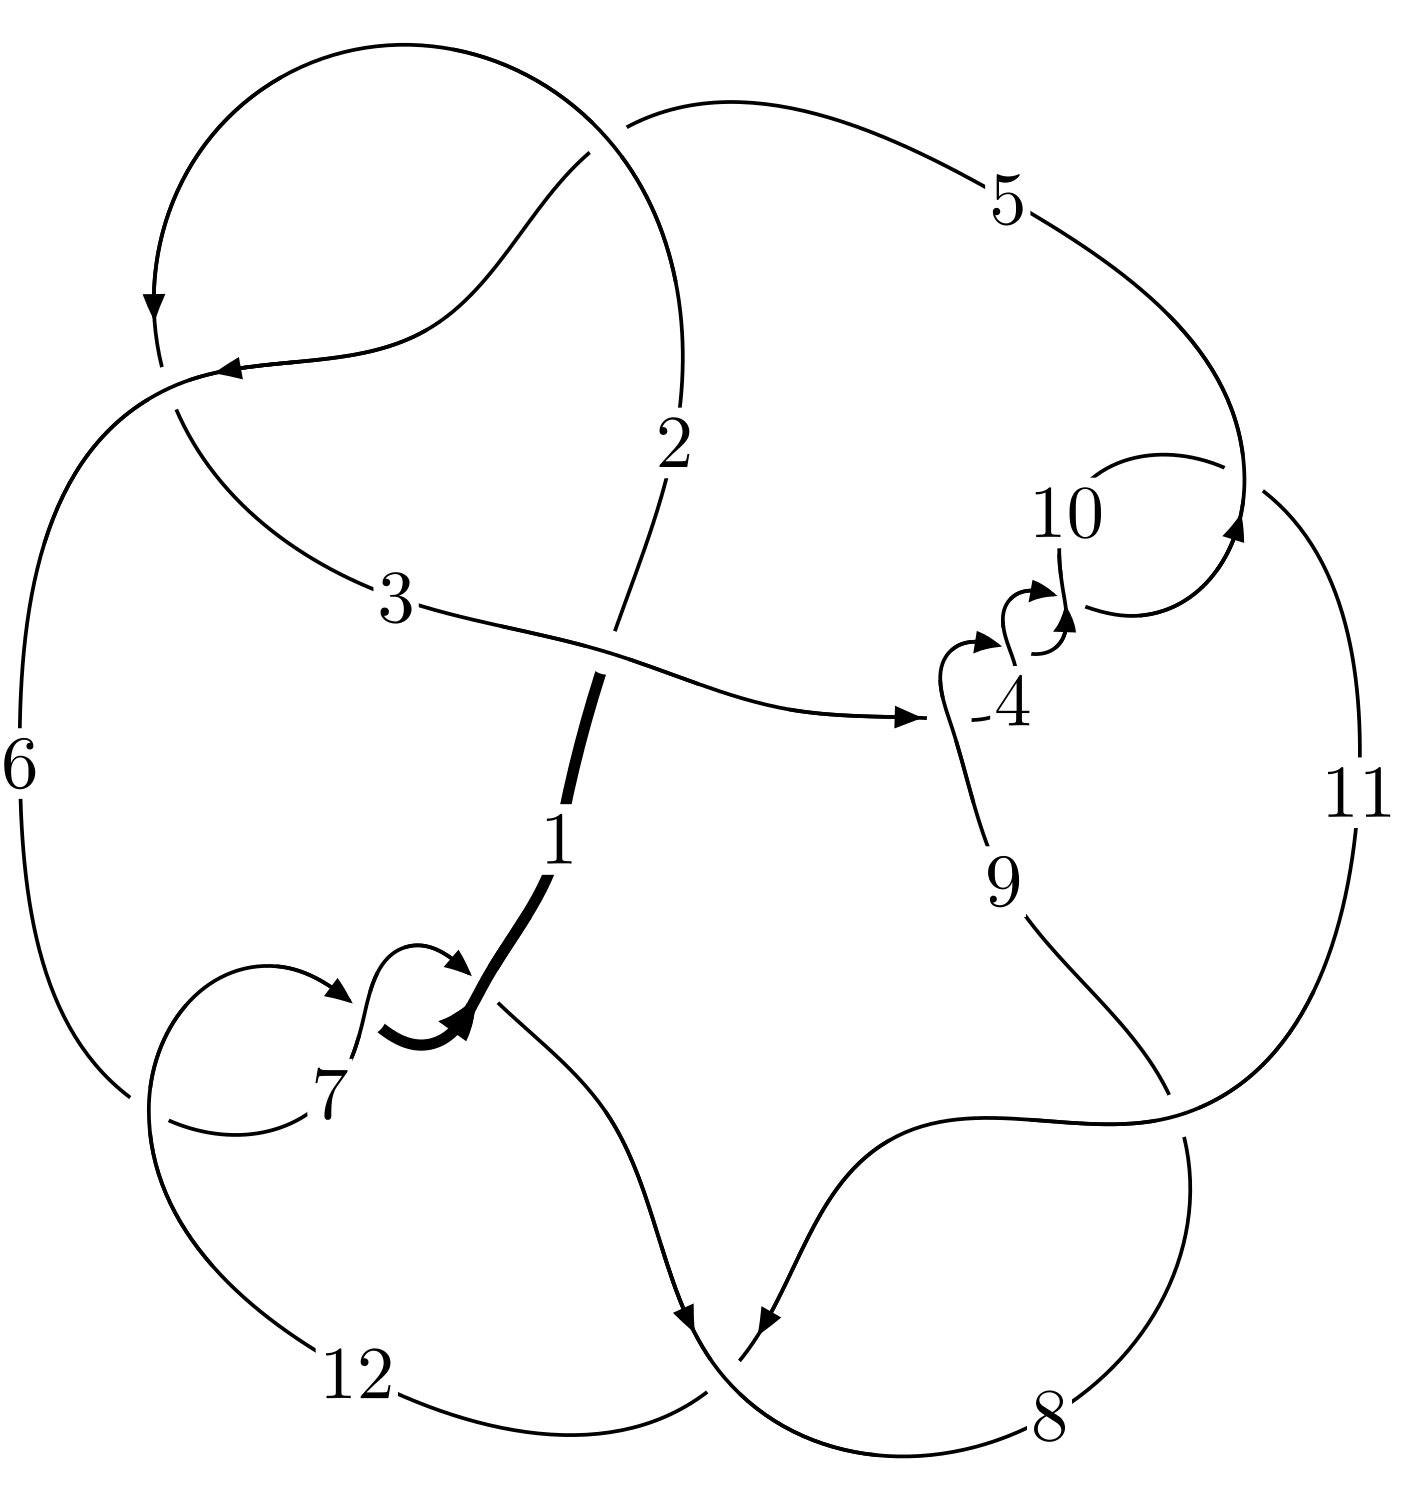
\includegraphics[width=112pt]{../../../GIT/diagram.site/Diagrams/png/1176_12a_0375.png}\\
\ \ \ A knot diagram\footnotemark}&
\allowdisplaybreaks
\textbf{Linearized knot diagam} \\
\cline{2-2}
 &
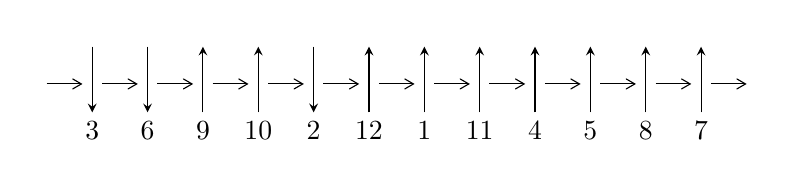
\begin{tikzpicture}[x=20pt, y=17pt]
	% nodes
	\node (C0) at (0, 0) {};
	\node (C1) at (1, 0) {};
	\node (C1U) at (1, +1) {};
	\node (C1D) at (1, -1) {3};

	\node (C2) at (2, 0) {};
	\node (C2U) at (2, +1) {};
	\node (C2D) at (2, -1) {6};

	\node (C3) at (3, 0) {};
	\node (C3U) at (3, +1) {};
	\node (C3D) at (3, -1) {9};

	\node (C4) at (4, 0) {};
	\node (C4U) at (4, +1) {};
	\node (C4D) at (4, -1) {10};

	\node (C5) at (5, 0) {};
	\node (C5U) at (5, +1) {};
	\node (C5D) at (5, -1) {2};

	\node (C6) at (6, 0) {};
	\node (C6U) at (6, +1) {};
	\node (C6D) at (6, -1) {12};

	\node (C7) at (7, 0) {};
	\node (C7U) at (7, +1) {};
	\node (C7D) at (7, -1) {1};

	\node (C8) at (8, 0) {};
	\node (C8U) at (8, +1) {};
	\node (C8D) at (8, -1) {11};

	\node (C9) at (9, 0) {};
	\node (C9U) at (9, +1) {};
	\node (C9D) at (9, -1) {4};

	\node (C10) at (10, 0) {};
	\node (C10U) at (10, +1) {};
	\node (C10D) at (10, -1) {5};

	\node (C11) at (11, 0) {};
	\node (C11U) at (11, +1) {};
	\node (C11D) at (11, -1) {8};

	\node (C12) at (12, 0) {};
	\node (C12U) at (12, +1) {};
	\node (C12D) at (12, -1) {7};
	\node (C13) at (13, 0) {};

	% arrows
	\draw[->,>={angle 60}]
	(C0) edge (C1) (C1) edge (C2) (C2) edge (C3) (C3) edge (C4) (C4) edge (C5) (C5) edge (C6) (C6) edge (C7) (C7) edge (C8) (C8) edge (C9) (C9) edge (C10) (C10) edge (C11) (C11) edge (C12) (C12) edge (C13) ;	\draw[->,>=stealth]
	(C1U) edge (C1D) (C2U) edge (C2D) (C3D) edge (C3U) (C4D) edge (C4U) (C5U) edge (C5D) (C6D) edge (C6U) (C7D) edge (C7U) (C8D) edge (C8U) (C9D) edge (C9U) (C10D) edge (C10U) (C11D) edge (C11U) (C12D) edge (C12U) ;
	\end{tikzpicture} \\
\hhline{~~} \\& 
\textbf{Solving Sequence} \\ \cline{2-2} 
 &
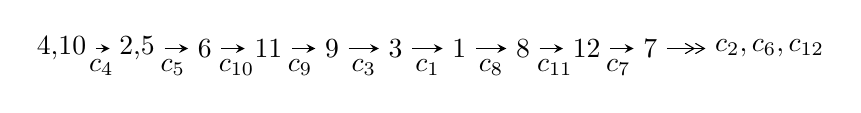
\begin{tikzpicture}[x=23pt, y=7pt]
	% node
	\node (A0) at (-1/8, 0) {4,10};
	\node (A1) at (17/16, 0) {2,5};
	\node (A2) at (17/8, 0) {6};
	\node (A3) at (25/8, 0) {11};
	\node (A4) at (33/8, 0) {9};
	\node (A5) at (41/8, 0) {3};
	\node (A6) at (49/8, 0) {1};
	\node (A7) at (57/8, 0) {8};
	\node (A8) at (65/8, 0) {12};
	\node (A9) at (73/8, 0) {7};
	\node (C1) at (1/2, -1) {$c_{4}$};
	\node (C2) at (13/8, -1) {$c_{5}$};
	\node (C3) at (21/8, -1) {$c_{10}$};
	\node (C4) at (29/8, -1) {$c_{9}$};
	\node (C5) at (37/8, -1) {$c_{3}$};
	\node (C6) at (45/8, -1) {$c_{1}$};
	\node (C7) at (53/8, -1) {$c_{8}$};
	\node (C8) at (61/8, -1) {$c_{11}$};
	\node (C9) at (69/8, -1) {$c_{7}$};
	\node (A10) at (11, 0) {$c_{2},c_{6},c_{12}$};

	% edge
	\draw[->,>=stealth]	
	(A0) edge (A1) (A1) edge (A2) (A2) edge (A3) (A3) edge (A4) (A4) edge (A5) (A5) edge (A6) (A6) edge (A7) (A7) edge (A8) (A8) edge (A9) ;
	\draw[->>,>={angle 60}]	
	(A9) edge (A10);
\end{tikzpicture} \\ 

\end{tabular} \\

\footnotetext{
The image of knot diagram is generated by the software ``\textbf{Draw programme}" developed by Andrew Bartholomew(\url{http://www.layer8.co.uk/maths/draw/index.htm\#Running-draw}), where we modified some parts for our purpose(\url{https://github.com/CATsTAILs/LinksPainter}).
}\phantom \\ \newline 
\centering \textbf{Ideals for irreducible components\footnotemark of $X_{\text{par}}$} 
 
\begin{align*}
I^u_{1}&=\langle 
-4 u^{42}+u^{41}+\cdots+4 b-4,\;2 u^{42}- u^{41}+\cdots+4 a-2,\;u^{43}-2 u^{42}+\cdots+2 u^2-2\rangle \\
I^u_{2}&=\langle 
2 u^5 a-2 u^5- a^2 u^2-8 u^3 a+2 u^2 a+8 u^3+2 a^2+8 a u-2 u^2+b-4 a-8 u+4,\\
\phantom{I^u_{2}}&\phantom{= \langle  }2 u^5 a^2- u^5 a-6 u^3 a^2+u^5+2 a^2 u^2+6 u^3 a+a^3+4 a^2 u- u^2 a-4 u^3-4 a^2-8 a u+u^2+5 a+4 u-3,\\
\phantom{I^u_{2}}&\phantom{= \langle  }u^6+u^5-3 u^4-2 u^3+2 u^2- u-1\rangle \\
I^u_{3}&=\langle 
b+u-1,\;2 a- u,\;u^2-2\rangle \\
\\
I^v_{1}&=\langle 
a,\;b+1,\;v-1\rangle \\
\end{align*}
\raggedright * 4 irreducible components of $\dim_{\mathbb{C}}=0$, with total 64 representations.\\
\footnotetext{All coefficients of polynomials are rational numbers. But the coefficients are sometimes approximated in decimal forms when there is not enough margin.}
\newpage
\renewcommand{\arraystretch}{1}
\centering \section*{I. $I^u_{1}= \langle -4 u^{42}+u^{41}+\cdots+4 b-4,\;2 u^{42}- u^{41}+\cdots+4 a-2,\;u^{43}-2 u^{42}+\cdots+2 u^2-2 \rangle$}
\flushleft \textbf{(i) Arc colorings}\\
\begin{tabular}{m{7pt} m{180pt} m{7pt} m{180pt} }
\flushright $a_{4}=$&$\begin{pmatrix}1\\0\end{pmatrix}$ \\
\flushright $a_{10}=$&$\begin{pmatrix}0\\u\end{pmatrix}$ \\
\flushright $a_{2}=$&$\begin{pmatrix}-\frac{1}{2} u^{42}+\frac{1}{4} u^{41}+\cdots-\frac{1}{2} u+\frac{1}{2}\\u^{42}-\frac{1}{4} u^{41}+\cdots+\frac{1}{2} u+1\end{pmatrix}$ \\
\flushright $a_{5}=$&$\begin{pmatrix}1\\- u^2\end{pmatrix}$ \\
\flushright $a_{6}=$&$\begin{pmatrix}\frac{1}{2} u^{42}-\frac{23}{2} u^{40}+\cdots+u^2+\frac{3}{2}\\- u^{42}+\frac{1}{4} u^{41}+\cdots-\frac{1}{2} u-1\end{pmatrix}$ \\
\flushright $a_{11}=$&$\begin{pmatrix}u\\- u^3+u\end{pmatrix}$ \\
\flushright $a_{9}=$&$\begin{pmatrix}- u\\u\end{pmatrix}$ \\
\flushright $a_{3}=$&$\begin{pmatrix}- u^2+1\\u^2\end{pmatrix}$ \\
\flushright $a_{1}=$&$\begin{pmatrix}-\frac{1}{2} u^{42}+\frac{21}{2} u^{40}+\cdots- u-\frac{1}{2}\\u^{42}-22 u^{40}+\cdots+\frac{1}{2} u+1\end{pmatrix}$ \\
\flushright $a_{8}=$&$\begin{pmatrix}u^5-2 u^3- u\\- u^7+3 u^5-2 u^3+u\end{pmatrix}$ \\
\flushright $a_{12}=$&$\begin{pmatrix}u^9-4 u^7+3 u^5+2 u^3+u\\- u^{11}+5 u^9-8 u^7+5 u^5-3 u^3+u\end{pmatrix}$ \\
\flushright $a_{7}=$&$\begin{pmatrix}\frac{1}{4} u^{32}-\frac{17}{4} u^{30}+\cdots-\frac{3}{2} u+\frac{1}{2}\\-\frac{1}{4} u^{32}+4 u^{30}+\cdots-\frac{1}{2} u^2+u\end{pmatrix}$\\&\end{tabular}
\flushleft \textbf{(ii) Obstruction class $= -1$}\\~\\
\flushleft \textbf{(iii) Cusp Shapes $= 2 u^{42}-46 u^{40}+\cdots-2 u+8$}\\~\\
\newpage\renewcommand{\arraystretch}{1}
\flushleft \textbf{(iv) u-Polynomials at the component}\newline \\
\begin{tabular}{m{50pt}|m{274pt}}
Crossings & \hspace{64pt}u-Polynomials at each crossing \\
\hline $$\begin{aligned}c_{1}\end{aligned}$$&$\begin{aligned}
&u^{43}+22 u^{42}+\cdots+9 u+1
\end{aligned}$\\
\hline $$\begin{aligned}c_{2},c_{5}\end{aligned}$$&$\begin{aligned}
&u^{43}+2 u^{42}+\cdots+u-1
\end{aligned}$\\
\hline $$\begin{aligned}c_{3},c_{4},c_{9}\\c_{10}\end{aligned}$$&$\begin{aligned}
&u^{43}+2 u^{42}+\cdots-2 u^2+2
\end{aligned}$\\
\hline $$\begin{aligned}c_{6},c_{7},c_{12}\end{aligned}$$&$\begin{aligned}
&u^{43}-2 u^{42}+\cdots-11 u-1
\end{aligned}$\\
\hline $$\begin{aligned}c_{8},c_{11}\end{aligned}$$&$\begin{aligned}
&u^{43}+6 u^{42}+\cdots+160 u+16
\end{aligned}$\\
\hline
\end{tabular}\\~\\
\newpage\renewcommand{\arraystretch}{1}
\flushleft \textbf{(v) Riley Polynomials at the component}\newline \\
\begin{tabular}{m{50pt}|m{274pt}}
Crossings & \hspace{64pt}Riley Polynomials at each crossing \\
\hline $$\begin{aligned}c_{1}\end{aligned}$$&$\begin{aligned}
&y^{43}+2 y^{42}+\cdots+53 y-1
\end{aligned}$\\
\hline $$\begin{aligned}c_{2},c_{5}\end{aligned}$$&$\begin{aligned}
&y^{43}-22 y^{42}+\cdots+9 y-1
\end{aligned}$\\
\hline $$\begin{aligned}c_{3},c_{4},c_{9}\\c_{10}\end{aligned}$$&$\begin{aligned}
&y^{43}-46 y^{42}+\cdots+8 y-4
\end{aligned}$\\
\hline $$\begin{aligned}c_{6},c_{7},c_{12}\end{aligned}$$&$\begin{aligned}
&y^{43}-38 y^{42}+\cdots+89 y-1
\end{aligned}$\\
\hline $$\begin{aligned}c_{8},c_{11}\end{aligned}$$&$\begin{aligned}
&y^{43}+30 y^{42}+\cdots+26112 y-256
\end{aligned}$\\
\hline
\end{tabular}\\~\\
\newpage\flushleft \textbf{(vi) Complex Volumes and Cusp Shapes}
$$\begin{array}{c|c|c}  
\text{Solutions to }I^u_{1}& \I (\text{vol} + \sqrt{-1}CS) & \text{Cusp shape}\\
 \hline 
\begin{aligned}
u &= \phantom{-}0.591746 + 0.636717 I \\
a &= -1.23572 - 1.63525 I \\
b &= -0.100756 + 0.318643 I\end{aligned}
 & -1.84282 + 10.94570 I & \phantom{-}6.30092 - 8.93673 I \\ \hline\begin{aligned}
u &= \phantom{-}0.591746 - 0.636717 I \\
a &= -1.23572 + 1.63525 I \\
b &= -0.100756 - 0.318643 I\end{aligned}
 & -1.84282 - 10.94570 I & \phantom{-}6.30092 + 8.93673 I \\ \hline\begin{aligned}
u &= -0.765729 + 0.373369 I \\
a &= -0.32757 + 1.59857 I \\
b &= \phantom{-}0.134514 - 0.340307 I\end{aligned}
 & \phantom{-}5.12970 - 5.35425 I & \phantom{-}12.2003 + 7.7214 I \\ \hline\begin{aligned}
u &= -0.765729 - 0.373369 I \\
a &= -0.32757 - 1.59857 I \\
b &= \phantom{-}0.134514 + 0.340307 I\end{aligned}
 & \phantom{-}5.12970 + 5.35425 I & \phantom{-}12.2003 - 7.7214 I \\ \hline\begin{aligned}
u &= \phantom{-}0.826606 + 0.202990 I \\
a &= \phantom{-}0.511476 + 0.581636 I \\
b &= \phantom{-}0.430064 + 0.050748 I\end{aligned}
 & \phantom{-}6.06160 + 0.79364 I & \phantom{-}14.9061 - 0.8864 I \\ \hline\begin{aligned}
u &= \phantom{-}0.826606 - 0.202990 I \\
a &= \phantom{-}0.511476 - 0.581636 I \\
b &= \phantom{-}0.430064 - 0.050748 I\end{aligned}
 & \phantom{-}6.06160 - 0.79364 I & \phantom{-}14.9061 + 0.8864 I \\ \hline\begin{aligned}
u &= -0.546701 + 0.616087 I \\
a &= -1.33752 + 1.76286 I \\
b &= -0.098208 - 0.285427 I\end{aligned}
 & -6.30176 - 6.51240 I & \phantom{-}1.84350 + 6.82731 I \\ \hline\begin{aligned}
u &= -0.546701 - 0.616087 I \\
a &= -1.33752 - 1.76286 I \\
b &= -0.098208 + 0.285427 I\end{aligned}
 & -6.30176 + 6.51240 I & \phantom{-}1.84350 - 6.82731 I \\ \hline\begin{aligned}
u &= -0.582396 + 0.579810 I \\
a &= \phantom{-}0.659858 - 0.192915 I \\
b &= \phantom{-}0.279952 - 0.384491 I\end{aligned}
 & \phantom{-}1.26998 - 5.99398 I & \phantom{-}9.54778 + 6.06507 I \\ \hline\begin{aligned}
u &= -0.582396 - 0.579810 I \\
a &= \phantom{-}0.659858 + 0.192915 I \\
b &= \phantom{-}0.279952 + 0.384491 I\end{aligned}
 & \phantom{-}1.26998 + 5.99398 I & \phantom{-}9.54778 - 6.06507 I\\
 \hline 
 \end{array}$$\newpage$$\begin{array}{c|c|c}  
\text{Solutions to }I^u_{1}& \I (\text{vol} + \sqrt{-1}CS) & \text{Cusp shape}\\
 \hline 
\begin{aligned}
u &= \phantom{-}0.403178 + 0.680325 I \\
a &= \phantom{-}0.873527 + 0.218379 I \\
b &= -0.795082 - 0.902473 I\end{aligned}
 & -2.40444 - 6.51462 I & \phantom{-}5.07632 + 3.55431 I \\ \hline\begin{aligned}
u &= \phantom{-}0.403178 - 0.680325 I \\
a &= \phantom{-}0.873527 - 0.218379 I \\
b &= -0.795082 + 0.902473 I\end{aligned}
 & -2.40444 + 6.51462 I & \phantom{-}5.07632 - 3.55431 I \\ \hline\begin{aligned}
u &= -0.443849 + 0.633747 I \\
a &= \phantom{-}0.902439 - 0.228432 I \\
b &= -0.888609 + 0.891580 I\end{aligned}
 & -6.60622 + 2.27578 I & \phantom{-}0.698054 - 0.385736 I \\ \hline\begin{aligned}
u &= -0.443849 - 0.633747 I \\
a &= \phantom{-}0.902439 + 0.228432 I \\
b &= -0.888609 - 0.891580 I\end{aligned}
 & -6.60622 - 2.27578 I & \phantom{-}0.698054 + 0.385736 I \\ \hline\begin{aligned}
u &= -0.377654 + 0.599705 I \\
a &= \phantom{-}0.738904 - 0.108280 I \\
b &= \phantom{-}0.103319 - 0.421977 I\end{aligned}
 & \phantom{-}0.67597 + 1.96643 I & \phantom{-}8.14582 + 0.08681 I \\ \hline\begin{aligned}
u &= -0.377654 - 0.599705 I \\
a &= \phantom{-}0.738904 + 0.108280 I \\
b &= \phantom{-}0.103319 + 0.421977 I\end{aligned}
 & \phantom{-}0.67597 - 1.96643 I & \phantom{-}8.14582 - 0.08681 I \\ \hline\begin{aligned}
u &= \phantom{-}1.34352\phantom{ +0.000000I} \\
a &= -0.457746\phantom{ +0.000000I} \\
b &= \phantom{-}1.25945\phantom{ +0.000000I}\end{aligned}
 & \phantom{-}6.42503\phantom{ +0.000000I} & \phantom{-}14.7720\phantom{ +0.000000I} \\ \hline\begin{aligned}
u &= \phantom{-}0.596066 + 0.273723 I \\
a &= \phantom{-}0.15234 - 2.25587 I \\
b &= \phantom{-}0.108473 + 0.195176 I\end{aligned}
 & -0.17994 + 3.15116 I & \phantom{-}7.13825 - 9.28828 I \\ \hline\begin{aligned}
u &= \phantom{-}0.596066 - 0.273723 I \\
a &= \phantom{-}0.15234 + 2.25587 I \\
b &= \phantom{-}0.108473 - 0.195176 I\end{aligned}
 & -0.17994 - 3.15116 I & \phantom{-}7.13825 + 9.28828 I \\ \hline\begin{aligned}
u &= -0.084134 + 0.604122 I \\
a &= \phantom{-}0.845349 - 0.074679 I \\
b &= -0.465947 + 0.534008 I\end{aligned}
 & \phantom{-}2.98218 + 1.98828 I & \phantom{-}8.33137 - 3.20557 I\\
 \hline 
 \end{array}$$\newpage$$\begin{array}{c|c|c}  
\text{Solutions to }I^u_{1}& \I (\text{vol} + \sqrt{-1}CS) & \text{Cusp shape}\\
 \hline 
\begin{aligned}
u &= -0.084134 - 0.604122 I \\
a &= \phantom{-}0.845349 + 0.074679 I \\
b &= -0.465947 - 0.534008 I\end{aligned}
 & \phantom{-}2.98218 - 1.98828 I & \phantom{-}8.33137 + 3.20557 I \\ \hline\begin{aligned}
u &= -1.43197\phantom{ +0.000000I} \\
a &= \phantom{-}0.0229961\phantom{ +0.000000I} \\
b &= \phantom{-}1.00111\phantom{ +0.000000I}\end{aligned}
 & \phantom{-}3.32572\phantom{ +0.000000I} & \phantom{-0.000000 } 0 \\ \hline\begin{aligned}
u &= -1.43137 + 0.20558 I \\
a &= \phantom{-}0.132330 - 0.142499 I \\
b &= \phantom{-}0.955154 - 0.077955 I\end{aligned}
 & \phantom{-}3.46742 + 3.34369 I & \phantom{-0.000000 } 0 \\ \hline\begin{aligned}
u &= -1.43137 - 0.20558 I \\
a &= \phantom{-}0.132330 + 0.142499 I \\
b &= \phantom{-}0.955154 + 0.077955 I\end{aligned}
 & \phantom{-}3.46742 - 3.34369 I & \phantom{-0.000000 } 0 \\ \hline\begin{aligned}
u &= \phantom{-}1.47158 + 0.11058 I \\
a &= -0.881376 - 0.770659 I \\
b &= \phantom{-}1.53453 + 1.36753 I\end{aligned}
 & \phantom{-}6.53226 + 0.41130 I & \phantom{-0.000000 } 0 \\ \hline\begin{aligned}
u &= \phantom{-}1.47158 - 0.11058 I \\
a &= -0.881376 + 0.770659 I \\
b &= \phantom{-}1.53453 - 1.36753 I\end{aligned}
 & \phantom{-}6.53226 - 0.41130 I & \phantom{-0.000000 } 0 \\ \hline\begin{aligned}
u &= \phantom{-}1.47924 + 0.17979 I \\
a &= \phantom{-}0.131246 + 0.108669 I \\
b &= \phantom{-}0.986913 + 0.072464 I\end{aligned}
 & -0.365210 + 0.609893 I & \phantom{-0.000000 } 0 \\ \hline\begin{aligned}
u &= \phantom{-}1.47924 - 0.17979 I \\
a &= \phantom{-}0.131246 - 0.108669 I \\
b &= \phantom{-}0.986913 - 0.072464 I\end{aligned}
 & -0.365210 - 0.609893 I & \phantom{-0.000000 } 0 \\ \hline\begin{aligned}
u &= -0.463968\phantom{ +0.000000I} \\
a &= \phantom{-}1.94534\phantom{ +0.000000I} \\
b &= \phantom{-}0.138255\phantom{ +0.000000I}\end{aligned}
 & \phantom{-}0.736315\phantom{ +0.000000I} & \phantom{-}13.7490\phantom{ +0.000000I} \\ \hline\begin{aligned}
u &= \phantom{-}1.53818 + 0.18818 I \\
a &= \phantom{-}0.21264 + 2.03609 I \\
b &= -0.50972 - 4.35591 I\end{aligned}
 & \phantom{-}0.59349 + 9.42918 I & \phantom{-0.000000 } 0\\
 \hline 
 \end{array}$$\newpage$$\begin{array}{c|c|c}  
\text{Solutions to }I^u_{1}& \I (\text{vol} + \sqrt{-1}CS) & \text{Cusp shape}\\
 \hline 
\begin{aligned}
u &= \phantom{-}1.53818 - 0.18818 I \\
a &= \phantom{-}0.21264 - 2.03609 I \\
b &= -0.50972 + 4.35591 I\end{aligned}
 & \phantom{-}0.59349 - 9.42918 I & \phantom{-0.000000 } 0 \\ \hline\begin{aligned}
u &= -1.55142 + 0.05723 I \\
a &= -0.80889 - 2.01985 I \\
b &= \phantom{-}1.44195 + 4.18487 I\end{aligned}
 & \phantom{-}7.05051 - 4.24670 I & \phantom{-0.000000 } 0 \\ \hline\begin{aligned}
u &= -1.55142 - 0.05723 I \\
a &= -0.80889 + 2.01985 I \\
b &= \phantom{-}1.44195 - 4.18487 I\end{aligned}
 & \phantom{-}7.05051 + 4.24670 I & \phantom{-0.000000 } 0 \\ \hline\begin{aligned}
u &= \phantom{-}1.55532 + 0.17621 I \\
a &= -0.711365 - 0.950566 I \\
b &= \phantom{-}0.99205 + 1.76418 I\end{aligned}
 & \phantom{-}8.38956 + 8.75469 I & \phantom{-0.000000 } 0 \\ \hline\begin{aligned}
u &= \phantom{-}1.55532 - 0.17621 I \\
a &= -0.711365 + 0.950566 I \\
b &= \phantom{-}0.99205 - 1.76418 I\end{aligned}
 & \phantom{-}8.38956 - 8.75469 I & \phantom{-0.000000 } 0 \\ \hline\begin{aligned}
u &= -1.55776 + 0.19984 I \\
a &= \phantom{-}0.19109 - 1.91237 I \\
b &= -0.48048 + 4.13035 I\end{aligned}
 & \phantom{-}5.2865 - 14.0160 I & \phantom{-0.000000 } 0 \\ \hline\begin{aligned}
u &= -1.55776 - 0.19984 I \\
a &= \phantom{-}0.19109 + 1.91237 I \\
b &= -0.48048 - 4.13035 I\end{aligned}
 & \phantom{-}5.2865 + 14.0160 I & \phantom{-0.000000 } 0 \\ \hline\begin{aligned}
u &= \phantom{-}0.155892 + 0.389253 I \\
a &= \phantom{-}0.939590 + 0.061625 I \\
b &= -0.782027 - 0.295786 I\end{aligned}
 & -1.51738 - 0.78597 I & -1.81615 + 1.01522 I \\ \hline\begin{aligned}
u &= \phantom{-}0.155892 - 0.389253 I \\
a &= \phantom{-}0.939590 - 0.061625 I \\
b &= -0.782027 + 0.295786 I\end{aligned}
 & -1.51738 + 0.78597 I & -1.81615 - 1.01522 I \\ \hline\begin{aligned}
u &= -1.60026 + 0.04435 I \\
a &= -0.79147 + 1.29002 I \\
b &= \phantom{-}1.26150 - 2.64623 I\end{aligned}
 & \phantom{-}14.2395 - 1.6305 I & \phantom{-0.000000 } 0\\
 \hline 
 \end{array}$$\newpage$$\begin{array}{c|c|c}  
\text{Solutions to }I^u_{1}& \I (\text{vol} + \sqrt{-1}CS) & \text{Cusp shape}\\
 \hline 
\begin{aligned}
u &= -1.60026 - 0.04435 I \\
a &= -0.79147 - 1.29002 I \\
b &= \phantom{-}1.26150 + 2.64623 I\end{aligned}
 & \phantom{-}14.2395 + 1.6305 I & \phantom{-0.000000 } 0 \\ \hline\begin{aligned}
u &= \phantom{-}1.59968 + 0.08511 I \\
a &= -0.45217 + 1.80198 I \\
b &= \phantom{-}0.69300 - 3.81498 I\end{aligned}
 & \phantom{-}13.1581 + 6.9538 I & \phantom{-0.000000 } 0 \\ \hline\begin{aligned}
u &= \phantom{-}1.59968 - 0.08511 I \\
a &= -0.45217 - 1.80198 I \\
b &= \phantom{-}0.69300 + 3.81498 I\end{aligned}
 & \phantom{-}13.1581 - 6.9538 I & \phantom{-0.000000 } 0\\
 \hline 
 \end{array}$$\newpage\newpage\renewcommand{\arraystretch}{1}
\centering \section*{II. $I^u_{2}= \langle 2 u^5 a-2 u^5+\cdots-4 a+4,\;2 u^5 a^2- u^5 a+\cdots+5 a-3,\;u^6+u^5-3 u^4-2 u^3+2 u^2- u-1 \rangle$}
\flushleft \textbf{(i) Arc colorings}\\
\begin{tabular}{m{7pt} m{180pt} m{7pt} m{180pt} }
\flushright $a_{4}=$&$\begin{pmatrix}1\\0\end{pmatrix}$ \\
\flushright $a_{10}=$&$\begin{pmatrix}0\\u\end{pmatrix}$ \\
\flushright $a_{2}=$&$\begin{pmatrix}a\\-2 u^5 a+2 u^5+\cdots+4 a-4\end{pmatrix}$ \\
\flushright $a_{5}=$&$\begin{pmatrix}1\\- u^2\end{pmatrix}$ \\
\flushright $a_{6}=$&$\begin{pmatrix}-2 u^5 a+2 u^5+\cdots+5 a-4\\2 u^5 a-2 u^5+\cdots-4 a+4\end{pmatrix}$ \\
\flushright $a_{11}=$&$\begin{pmatrix}u\\- u^3+u\end{pmatrix}$ \\
\flushright $a_{9}=$&$\begin{pmatrix}- u\\u\end{pmatrix}$ \\
\flushright $a_{3}=$&$\begin{pmatrix}- u^2+1\\u^2\end{pmatrix}$ \\
\flushright $a_{1}=$&$\begin{pmatrix}- u^5 a^2-2 u^5 a+\cdots- a^2+a\\u^5 a^2-2 u^5 a+\cdots+6 a-6\end{pmatrix}$ \\
\flushright $a_{8}=$&$\begin{pmatrix}u^5-2 u^3- u\\- u^5+u^4+2 u^3-3 u^2+u+1\end{pmatrix}$ \\
\flushright $a_{12}=$&$\begin{pmatrix}u^2-1\\- u^2\end{pmatrix}$ \\
\flushright $a_{7}=$&$\begin{pmatrix}u^4 a^2+u^4 a-2 a^2 u^2-3 u^2 a+2 u^2+3 a-2\\2 u^5 a-2 u^5+\cdots-6 a+6\end{pmatrix}$\\&\end{tabular}
\flushleft \textbf{(ii) Obstruction class $= -1$}\\~\\
\flushleft \textbf{(iii) Cusp Shapes $= 4 u^3-8 u+10$}\\~\\
\newpage\renewcommand{\arraystretch}{1}
\flushleft \textbf{(iv) u-Polynomials at the component}\newline \\
\begin{tabular}{m{50pt}|m{274pt}}
Crossings & \hspace{64pt}u-Polynomials at each crossing \\
\hline $$\begin{aligned}c_{1}\end{aligned}$$&$\begin{aligned}
&u^{18}+12 u^{17}+\cdots+5 u+1
\end{aligned}$\\
\hline $$\begin{aligned}c_{2},c_{5},c_{6}\\c_{7},c_{12}\end{aligned}$$&$\begin{aligned}
&u^{18}-6 u^{16}+\cdots+u-1
\end{aligned}$\\
\hline $$\begin{aligned}c_{3},c_{4},c_{9}\\c_{10}\end{aligned}$$&$\begin{aligned}
&(u^6- u^5-3 u^4+2 u^3+2 u^2+u-1)^3
\end{aligned}$\\
\hline $$\begin{aligned}c_{8},c_{11}\end{aligned}$$&$\begin{aligned}
&(u^6+u^5+3 u^4+2 u^3+2 u^2+u-1)^3
\end{aligned}$\\
\hline
\end{tabular}\\~\\
\newpage\renewcommand{\arraystretch}{1}
\flushleft \textbf{(v) Riley Polynomials at the component}\newline \\
\begin{tabular}{m{50pt}|m{274pt}}
Crossings & \hspace{64pt}Riley Polynomials at each crossing \\
\hline $$\begin{aligned}c_{1}\end{aligned}$$&$\begin{aligned}
&y^{18}-12 y^{17}+\cdots-17 y+1
\end{aligned}$\\
\hline $$\begin{aligned}c_{2},c_{5},c_{6}\\c_{7},c_{12}\end{aligned}$$&$\begin{aligned}
&y^{18}-12 y^{17}+\cdots-5 y+1
\end{aligned}$\\
\hline $$\begin{aligned}c_{3},c_{4},c_{9}\\c_{10}\end{aligned}$$&$\begin{aligned}
&(y^6-7 y^5+17 y^4-16 y^3+6 y^2-5 y+1)^3
\end{aligned}$\\
\hline $$\begin{aligned}c_{8},c_{11}\end{aligned}$$&$\begin{aligned}
&(y^6+5 y^5+9 y^4+4 y^3-6 y^2-5 y+1)^3
\end{aligned}$\\
\hline
\end{tabular}\\~\\
\newpage\flushleft \textbf{(vi) Complex Volumes and Cusp Shapes}
$$\begin{array}{c|c|c}  
\text{Solutions to }I^u_{2}& \I (\text{vol} + \sqrt{-1}CS) & \text{Cusp shape}\\
 \hline 
\begin{aligned}
u &= \phantom{-}0.493180 + 0.575288 I \\
a &= \phantom{-}0.941013 + 0.239784 I \\
b &= -1.009960 - 0.876429 I\end{aligned}
 & -2.96024 + 1.97241 I & \phantom{-}4.57572 - 3.68478 I \\ \hline\begin{aligned}
u &= \phantom{-}0.493180 + 0.575288 I \\
a &= \phantom{-}0.703854 + 0.163676 I \\
b &= \phantom{-}0.204229 + 0.389849 I\end{aligned}
 & -2.96024 + 1.97241 I & \phantom{-}4.57572 - 3.68478 I \\ \hline\begin{aligned}
u &= \phantom{-}0.493180 + 0.575288 I \\
a &= -1.46493 - 2.00338 I \\
b &= -0.086351 + 0.244114 I\end{aligned}
 & -2.96024 + 1.97241 I & \phantom{-}4.57572 - 3.68478 I \\ \hline\begin{aligned}
u &= \phantom{-}0.493180 - 0.575288 I \\
a &= \phantom{-}0.941013 - 0.239784 I \\
b &= -1.009960 + 0.876429 I\end{aligned}
 & -2.96024 - 1.97241 I & \phantom{-}4.57572 + 3.68478 I \\ \hline\begin{aligned}
u &= \phantom{-}0.493180 - 0.575288 I \\
a &= \phantom{-}0.703854 - 0.163676 I \\
b &= \phantom{-}0.204229 - 0.389849 I\end{aligned}
 & -2.96024 - 1.97241 I & \phantom{-}4.57572 + 3.68478 I \\ \hline\begin{aligned}
u &= \phantom{-}0.493180 - 0.575288 I \\
a &= -1.46493 + 2.00338 I \\
b &= -0.086351 - 0.244114 I\end{aligned}
 & -2.96024 - 1.97241 I & \phantom{-}4.57572 + 3.68478 I \\ \hline\begin{aligned}
u &= -0.483672\phantom{ +0.000000I} \\
a &= \phantom{-}1.12121\phantom{ +0.000000I} \\
b &= -1.42631\phantom{ +0.000000I}\end{aligned}
 & \phantom{-}0.738851\phantom{ +0.000000I} & \phantom{-}13.4170\phantom{ +0.000000I} \\ \hline\begin{aligned}
u &= -0.483672\phantom{ +0.000000I} \\
a &= \phantom{-}1.85982 + 0.59462 I \\
b &= \phantom{-}0.146924 - 0.011821 I\end{aligned}
 & \phantom{-}0.738851\phantom{ +0.000000I} & \phantom{-}13.4170\phantom{ +0.000000I} \\ \hline\begin{aligned}
u &= -0.483672\phantom{ +0.000000I} \\
a &= \phantom{-}1.85982 - 0.59462 I \\
b &= \phantom{-}0.146924 + 0.011821 I\end{aligned}
 & \phantom{-}0.738851\phantom{ +0.000000I} & \phantom{-}13.4170\phantom{ +0.000000I} \\ \hline\begin{aligned}
u &= -1.52087 + 0.16310 I \\
a &= -0.751848 + 0.903227 I \\
b &= \phantom{-}1.13095 - 1.63417 I\end{aligned}
 & \phantom{-}3.69558 - 4.59213 I & \phantom{-}8.58114 + 3.20482 I\\
 \hline 
 \end{array}$$\newpage$$\begin{array}{c|c|c}  
\text{Solutions to }I^u_{2}& \I (\text{vol} + \sqrt{-1}CS) & \text{Cusp shape}\\
 \hline 
\begin{aligned}
u &= -1.52087 + 0.16310 I \\
a &= \phantom{-}0.137996 - 0.084846 I \\
b &= \phantom{-}1.011050 - 0.070016 I\end{aligned}
 & \phantom{-}3.69558 - 4.59213 I & \phantom{-}8.58114 + 3.20482 I \\ \hline\begin{aligned}
u &= -1.52087 + 0.16310 I \\
a &= \phantom{-}0.15868 - 2.23953 I \\
b &= -0.39625 + 4.72775 I\end{aligned}
 & \phantom{-}3.69558 - 4.59213 I & \phantom{-}8.58114 + 3.20482 I \\ \hline\begin{aligned}
u &= -1.52087 - 0.16310 I \\
a &= -0.751848 - 0.903227 I \\
b &= \phantom{-}1.13095 + 1.63417 I\end{aligned}
 & \phantom{-}3.69558 + 4.59213 I & \phantom{-}8.58114 - 3.20482 I \\ \hline\begin{aligned}
u &= -1.52087 - 0.16310 I \\
a &= \phantom{-}0.137996 + 0.084846 I \\
b &= \phantom{-}1.011050 + 0.070016 I\end{aligned}
 & \phantom{-}3.69558 + 4.59213 I & \phantom{-}8.58114 - 3.20482 I \\ \hline\begin{aligned}
u &= -1.52087 - 0.16310 I \\
a &= \phantom{-}0.15868 + 2.23953 I \\
b &= -0.39625 - 4.72775 I\end{aligned}
 & \phantom{-}3.69558 + 4.59213 I & \phantom{-}8.58114 - 3.20482 I \\ \hline\begin{aligned}
u &= \phantom{-}1.53904\phantom{ +0.000000I} \\
a &= \phantom{-}0.110457\phantom{ +0.000000I} \\
b &= \phantom{-}1.03249\phantom{ +0.000000I}\end{aligned}
 & \phantom{-}7.66009\phantom{ +0.000000I} & \phantom{-}12.2690\phantom{ +0.000000I} \\ \hline\begin{aligned}
u &= \phantom{-}1.53904\phantom{ +0.000000I} \\
a &= -1.20042 + 1.54308 I \\
b &= \phantom{-}2.19632 - 3.14900 I\end{aligned}
 & \phantom{-}7.66009\phantom{ +0.000000I} & \phantom{-}12.2690\phantom{ +0.000000I} \\ \hline\begin{aligned}
u &= \phantom{-}1.53904\phantom{ +0.000000I} \\
a &= -1.20042 - 1.54308 I \\
b &= \phantom{-}2.19632 + 3.14900 I\end{aligned}
 & \phantom{-}7.66009\phantom{ +0.000000I} & \phantom{-}12.2690\phantom{ +0.000000I}\\
 \hline 
 \end{array}$$\newpage\newpage\renewcommand{\arraystretch}{1}
\centering \section*{III. $I^u_{3}= \langle b+u-1,\;2 a- u,\;u^2-2 \rangle$}
\flushleft \textbf{(i) Arc colorings}\\
\begin{tabular}{m{7pt} m{180pt} m{7pt} m{180pt} }
\flushright $a_{4}=$&$\begin{pmatrix}1\\0\end{pmatrix}$ \\
\flushright $a_{10}=$&$\begin{pmatrix}0\\u\end{pmatrix}$ \\
\flushright $a_{2}=$&$\begin{pmatrix}\frac{1}{2} u\\- u+1\end{pmatrix}$ \\
\flushright $a_{5}=$&$\begin{pmatrix}1\\-2\end{pmatrix}$ \\
\flushright $a_{6}=$&$\begin{pmatrix}\frac{1}{2} u+1\\- u-1\end{pmatrix}$ \\
\flushright $a_{11}=$&$\begin{pmatrix}u\\- u\end{pmatrix}$ \\
\flushright $a_{9}=$&$\begin{pmatrix}- u\\u\end{pmatrix}$ \\
\flushright $a_{3}=$&$\begin{pmatrix}-1\\2\end{pmatrix}$ \\
\flushright $a_{1}=$&$\begin{pmatrix}\frac{1}{2} u+1\\- u-1\end{pmatrix}$ \\
\flushright $a_{8}=$&$\begin{pmatrix}- u\\u\end{pmatrix}$ \\
\flushright $a_{12}=$&$\begin{pmatrix}u\\- u\end{pmatrix}$ \\
\flushright $a_{7}=$&$\begin{pmatrix}-\frac{1}{2} u+1\\-1\end{pmatrix}$\\&\end{tabular}
\flushleft \textbf{(ii) Obstruction class $= 1$}\\~\\
\flushleft \textbf{(iii) Cusp Shapes $= 8$}\\~\\
\newpage\renewcommand{\arraystretch}{1}
\flushleft \textbf{(iv) u-Polynomials at the component}\newline \\
\begin{tabular}{m{50pt}|m{274pt}}
Crossings & \hspace{64pt}u-Polynomials at each crossing \\
\hline $$\begin{aligned}c_{1},c_{5},c_{6}\\c_{7}\end{aligned}$$&$\begin{aligned}
&(u-1)^2
\end{aligned}$\\
\hline $$\begin{aligned}c_{2},c_{12}\end{aligned}$$&$\begin{aligned}
&(u+1)^2
\end{aligned}$\\
\hline $$\begin{aligned}c_{3},c_{4},c_{9}\\c_{10}\end{aligned}$$&$\begin{aligned}
&u^2-2
\end{aligned}$\\
\hline $$\begin{aligned}c_{8},c_{11}\end{aligned}$$&$\begin{aligned}
&u^2
\end{aligned}$\\
\hline
\end{tabular}\\~\\
\newpage\renewcommand{\arraystretch}{1}
\flushleft \textbf{(v) Riley Polynomials at the component}\newline \\
\begin{tabular}{m{50pt}|m{274pt}}
Crossings & \hspace{64pt}Riley Polynomials at each crossing \\
\hline $$\begin{aligned}c_{1},c_{2},c_{5}\\c_{6},c_{7},c_{12}\end{aligned}$$&$\begin{aligned}
&(y-1)^2
\end{aligned}$\\
\hline $$\begin{aligned}c_{3},c_{4},c_{9}\\c_{10}\end{aligned}$$&$\begin{aligned}
&(y-2)^2
\end{aligned}$\\
\hline $$\begin{aligned}c_{8},c_{11}\end{aligned}$$&$\begin{aligned}
&y^2
\end{aligned}$\\
\hline
\end{tabular}\\~\\
\newpage\flushleft \textbf{(vi) Complex Volumes and Cusp Shapes}
$$\begin{array}{c|c|c}  
\text{Solutions to }I^u_{3}& \I (\text{vol} + \sqrt{-1}CS) & \text{Cusp shape}\\
 \hline 
\begin{aligned}
u &= \phantom{-}1.41421\phantom{ +0.000000I} \\
a &= \phantom{-}0.707107\phantom{ +0.000000I} \\
b &= -0.414214\phantom{ +0.000000I}\end{aligned}
 & \phantom{-}4.93480\phantom{ +0.000000I} & \phantom{-}8.00000\phantom{ +0.000000I} \\ \hline\begin{aligned}
u &= -1.41421\phantom{ +0.000000I} \\
a &= -0.707107\phantom{ +0.000000I} \\
b &= \phantom{-}2.41421\phantom{ +0.000000I}\end{aligned}
 & \phantom{-}4.93480\phantom{ +0.000000I} & \phantom{-}8.00000\phantom{ +0.000000I}\\
 \hline 
 \end{array}$$\newpage\newpage\renewcommand{\arraystretch}{1}
\centering \section*{IV. $I^v_{1}= \langle a,\;b+1,\;v-1 \rangle$}
\flushleft \textbf{(i) Arc colorings}\\
\begin{tabular}{m{7pt} m{180pt} m{7pt} m{180pt} }
\flushright $a_{4}=$&$\begin{pmatrix}1\\0\end{pmatrix}$ \\
\flushright $a_{10}=$&$\begin{pmatrix}1\\0\end{pmatrix}$ \\
\flushright $a_{2}=$&$\begin{pmatrix}0\\-1\end{pmatrix}$ \\
\flushright $a_{5}=$&$\begin{pmatrix}1\\0\end{pmatrix}$ \\
\flushright $a_{6}=$&$\begin{pmatrix}1\\1\end{pmatrix}$ \\
\flushright $a_{11}=$&$\begin{pmatrix}1\\0\end{pmatrix}$ \\
\flushright $a_{9}=$&$\begin{pmatrix}1\\0\end{pmatrix}$ \\
\flushright $a_{3}=$&$\begin{pmatrix}1\\0\end{pmatrix}$ \\
\flushright $a_{1}=$&$\begin{pmatrix}-1\\-1\end{pmatrix}$ \\
\flushright $a_{8}=$&$\begin{pmatrix}1\\0\end{pmatrix}$ \\
\flushright $a_{12}=$&$\begin{pmatrix}1\\0\end{pmatrix}$ \\
\flushright $a_{7}=$&$\begin{pmatrix}2\\1\end{pmatrix}$\\&\end{tabular}
\flushleft \textbf{(ii) Obstruction class $= 1$}\\~\\
\flushleft \textbf{(iii) Cusp Shapes $= 0$}\\~\\
\newpage\renewcommand{\arraystretch}{1}
\flushleft \textbf{(iv) u-Polynomials at the component}\newline \\
\begin{tabular}{m{50pt}|m{274pt}}
Crossings & \hspace{64pt}u-Polynomials at each crossing \\
\hline $$\begin{aligned}c_{1},c_{2},c_{12}\end{aligned}$$&$\begin{aligned}
&u-1
\end{aligned}$\\
\hline $$\begin{aligned}c_{3},c_{4},c_{8}\\c_{9},c_{10},c_{11}\end{aligned}$$&$\begin{aligned}
&u
\end{aligned}$\\
\hline $$\begin{aligned}c_{5},c_{6},c_{7}\end{aligned}$$&$\begin{aligned}
&u+1
\end{aligned}$\\
\hline
\end{tabular}\\~\\
\newpage\renewcommand{\arraystretch}{1}
\flushleft \textbf{(v) Riley Polynomials at the component}\newline \\
\begin{tabular}{m{50pt}|m{274pt}}
Crossings & \hspace{64pt}Riley Polynomials at each crossing \\
\hline $$\begin{aligned}c_{1},c_{2},c_{5}\\c_{6},c_{7},c_{12}\end{aligned}$$&$\begin{aligned}
&y-1
\end{aligned}$\\
\hline $$\begin{aligned}c_{3},c_{4},c_{8}\\c_{9},c_{10},c_{11}\end{aligned}$$&$\begin{aligned}
&y
\end{aligned}$\\
\hline
\end{tabular}\\~\\
\newpage\flushleft \textbf{(vi) Complex Volumes and Cusp Shapes}
$$\begin{array}{c|c|c}  
\text{Solutions to }I^v_{1}& \I (\text{vol} + \sqrt{-1}CS) & \text{Cusp shape}\\
 \hline 
\begin{aligned}
v &= \phantom{-}1.00000\phantom{ +0.000000I} \\
a &= \phantom{-0.000000 } 0 \\
b &= -1.00000\phantom{ +0.000000I}\end{aligned}
 & \phantom{-0.000000 } 0 & \phantom{-0.000000 } 0\\
 \hline 
 \end{array}$$\newpage
\newpage\renewcommand{\arraystretch}{1}
\centering \section*{ V. u-Polynomials}
\begin{tabular}{m{50pt}|m{274pt}}
Crossings & \hspace{64pt}u-Polynomials at each crossing \\
\hline $$\begin{aligned}c_{1}\end{aligned}$$&$\begin{aligned}
&((u-1)^3)(u^{18}+12 u^{17}+\cdots+5 u+1)(u^{43}+22 u^{42}+\cdots+9 u+1)
\end{aligned}$\\
\hline $$\begin{aligned}c_{2}\end{aligned}$$&$\begin{aligned}
&(u-1)(u+1)^2(u^{18}-6 u^{16}+\cdots+u-1)(u^{43}+2 u^{42}+\cdots+u-1)
\end{aligned}$\\
\hline $$\begin{aligned}c_{3},c_{4},c_{9}\\c_{10}\end{aligned}$$&$\begin{aligned}
&u(u^2-2)(u^6- u^5+\cdots+u-1)^{3}(u^{43}+2 u^{42}+\cdots-2 u^{2}+2)
\end{aligned}$\\
\hline $$\begin{aligned}c_{5}\end{aligned}$$&$\begin{aligned}
&((u-1)^2)(u+1)(u^{18}-6 u^{16}+\cdots+u-1)(u^{43}+2 u^{42}+\cdots+u-1)
\end{aligned}$\\
\hline $$\begin{aligned}c_{6},c_{7}\end{aligned}$$&$\begin{aligned}
&((u-1)^2)(u+1)(u^{18}-6 u^{16}+\cdots+u-1)(u^{43}-2 u^{42}+\cdots-11 u-1)
\end{aligned}$\\
\hline $$\begin{aligned}c_{8},c_{11}\end{aligned}$$&$\begin{aligned}
&u^3(u^6+u^5+\cdots+u-1)^{3}(u^{43}+6 u^{42}+\cdots+160 u+16)
\end{aligned}$\\
\hline $$\begin{aligned}c_{12}\end{aligned}$$&$\begin{aligned}
&(u-1)(u+1)^2(u^{18}-6 u^{16}+\cdots+u-1)(u^{43}-2 u^{42}+\cdots-11 u-1)
\end{aligned}$\\
\hline
\end{tabular}\newpage\renewcommand{\arraystretch}{1}
\centering \section*{ VI. Riley Polynomials}
\begin{tabular}{m{50pt}|m{274pt}}
Crossings & \hspace{64pt}Riley Polynomials at each crossing \\
\hline $$\begin{aligned}c_{1}\end{aligned}$$&$\begin{aligned}
&((y-1)^3)(y^{18}-12 y^{17}+\cdots-17 y+1)(y^{43}+2 y^{42}+\cdots+53 y-1)
\end{aligned}$\\
\hline $$\begin{aligned}c_{2},c_{5}\end{aligned}$$&$\begin{aligned}
&((y-1)^3)(y^{18}-12 y^{17}+\cdots-5 y+1)(y^{43}-22 y^{42}+\cdots+9 y-1)
\end{aligned}$\\
\hline $$\begin{aligned}c_{3},c_{4},c_{9}\\c_{10}\end{aligned}$$&$\begin{aligned}
&y(y-2)^2(y^6-7 y^5+17 y^4-16 y^3+6 y^2-5 y+1)^3\\
&\cdot(y^{43}-46 y^{42}+\cdots+8 y-4)
\end{aligned}$\\
\hline $$\begin{aligned}c_{6},c_{7},c_{12}\end{aligned}$$&$\begin{aligned}
&((y-1)^3)(y^{18}-12 y^{17}+\cdots-5 y+1)(y^{43}-38 y^{42}+\cdots+89 y-1)
\end{aligned}$\\
\hline $$\begin{aligned}c_{8},c_{11}\end{aligned}$$&$\begin{aligned}
&y^3(y^6+5 y^5+9 y^4+4 y^3-6 y^2-5 y+1)^3\\
&\cdot(y^{43}+30 y^{42}+\cdots+26112 y-256)
\end{aligned}$\\
\hline
\end{tabular}
\vskip 2pc
\end{document}